\documentclass[english]{thesis}
\usepackage[cpp]{mypackage}

\title{Homework 2}
\school{School of Data and Computer Science}
\author{Hongzheng Chen}
\stunum{17341015}
\headercontext{Parallel and Distributed Computing}

\begin{document}

\maketitle

\textbf{I think this homework exists lots of uncertainty.
We do not know what techniques in \emph{modern CPU} should be considered.
Like forwarding and superscalar, though the problem is not explictly mentioned, but they are both very important techniques in \emph{modern} CPU.
Moreover, only providing the machine configuration is not enough, the compiler can also affect the performance.
If some compiler techniques like loop unrolling or software pipelining are used, the results will be different.
Thus, I can only provide the answer in my understanding.}

\section{Instruction-Level Parallelism}
Suppose you have a machine $M_1$ with two load/store units that can each load or store a single value on each clock cycle, and one arithmetic unit that can perform one arithmetic operation (e.g., multiplication or addition) on each clock cycle.

\begin{itemize}
\item[A.] Assume that the load/store and arithmetic units have latencies of one cycle.
How many clock cycles would be required to execute \verb'computeInnerProduct' as a function of $N$?
Explain what limits the performance.

\bigskip
\textit{Answer.} We label the instructions as following.
\begin{lstlisting}
inline void innerProduct (point *a, point *b, float *result)
{
	float x1 = a->x; // 1, load from memory
	float x2 = b->x; // 2
	float product1 = x1*x2; // 3, store in register
	float y1 = a->y; // 4
	float y2 = b->y; // 5
	float product2 = y1*y2; // 6
	float inner = product1 + product2; // 7
	*result = inner; // 8
}
\end{lstlisting}

If no parallelism is considered, 4 loads, 2 multiplications, 1 addition and 1 store need 8 cycles per loop.
Thus, $8N$ cycles for \verb'computeInnerProduct'.

One cycle issuing one instruction limits the performance.

% Since there are only two load/store units and one arithmetic unit, we can obatin the optimal data flow graph, shown in Fig.~\ref{fig:dfg}.
% Notice the dependency relation should preserve.
% \begin{figure}[H]
% \centering
% 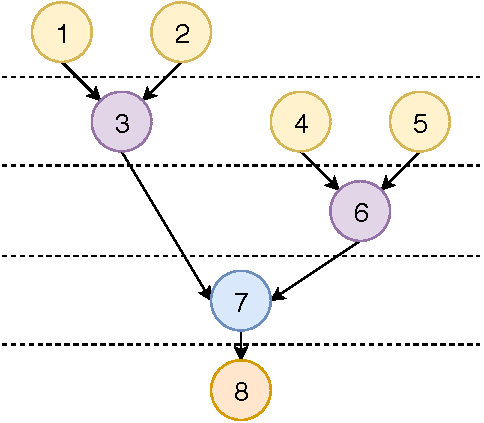
\includegraphics[width=0.3\linewidth]{fig/parallel-data-flow-graph.pdf}
% \caption{Data flow graph}
% \label{fig:dfg}
% \end{figure}

% From Fig.~\ref{fig:dfg}, we can clearly see that one \verb'innerProduct' needs $5$ cycles to compute at least.
% And two \verb'innerProduct's must be separated by $2$ cycles, since there are only two load/store units.

% Clearly, I/O (memory access) limits the performance.

\bigskip
\item[B.] Now assume that the load/store and arithmetic unit have latencies of 10 clock cycles,
but they are fully pipelined, able to initiate new operations every clock cycle.
How many clock cycles would be required to execute \verb'computeInnerProduct' as a function of N?
Explain how this relates to your answer to part A.

\bigskip
\textit{Answer.} Assume no forwarding is considered.
Since there are two load/store units, the 2nd instruction can be issued in the 2nd cycle.
But the third one should be wait for the first two instructions due to the dependency relation.
Then, 1+10+10=21 cycles are needed for the first three.

Although out-of-order execution is allowed, the limitation of load/store units does not allow the 4th and 5th instruction to be executed simultaneously.
Therefore, 21 cycles are also needed for 4$\to$6 instructions.

Since the load/store units are free after the first 10 cycles, the first load/store can be used in the 11th cycle, and the second one can be used in the 12th cycle.
That is to say, the 4th and 5th instruction can be hided behind the execution of $1\thicksim 3$ instructions (See Fig.~\ref{fig:execution}).
\begin{figure}[H]
\centering
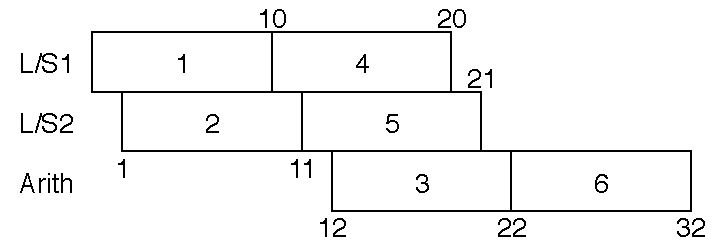
\includegraphics[width=0.6\linewidth]{parallel-execution.pdf}
\caption{Execution graph of Part B}
\label{fig:execution}
\end{figure}

In total, (21+1+10+10+10)N=52N cycles are required to execute \verb'computeInnerProduct'.

Part B is able to initiate new operations every clock cycle, thus the performance imporves.
The new limitation is the number of I/O ports.

\bigskip
\end{itemize}

\section{SIMD with ISPC}
Suppose machine $M_2$ has one 8-wide SIMD load/store unit, and one 8-wide SIMD arithmetic unit.
Both have latencies of one clock cycle.
\begin{itemize}
\item[A.] How many clock cycles would be required to execute \verb'computeInnerProductISPC' as a function of N?
Explain what limits the performance.

\bigskip
\textit{Answer.}
\begin{itemize}
\item Loading \verb'A[i].x', \verb'B[i].x', \verb'A[i].y', \verb'B[i].y' needs one cycle.
\item Adding two terms needs one cycle.
\item Storing the result into \verb'result[i]' needs one cycle.
\end{itemize}
Thus, each loop needs $3$ cycles to execute.
Notice the loop is \verb'foreach' loop.
If the machine has enough CPU cores and compiler fully parallelizes this loop, ignoring the threads creating overheads, then only $3$ cycles are needed for the whole loop, since no dependency relation among different loop index.

If the compiler just views the \verb'foreach' loop as \verb'for' loop, then $3N$ cycles are needed.

For other cases, I cannot figure out the results due to the lack of information.

\bigskip
\item[B.] If we were to run the \verb'computeInnerProductISPC' on a five-core machine $M_3$, where each core has the same SIMD capabilites as $M_2$, what would be the best speedup it could achieve over the single-core performance of part A?
Explain.

\bigskip
\textit{Answer.}
We can divide the task into 5 subtasks, say $0\thicksim N/5$ for core 1, $N/5\thicksim 2/5N$ for core 2, $\ldots$, $4/5N\thicksim N$ for core 5.
Since the SIMD capability in each core is the same, the best speedup would be 5x.

\bigskip
\end{itemize}

\section{Parallel Fractal Generation Using Pthreads}
Experimental setting:
\begin{itemize}
	\item Ubuntu 18.04(LTS) + gcc 7.3.0
	\item Intel Core i7-7700HQ 2.80GHz (8 cores)
	\item 8GB memory
\end{itemize}

For detailed implementation, please refer the codes in \verb'mandelbrot.cpp'.

Due to space limitation, only the output of 8 threads is shown in Fig.~\ref{fig:result}.
Other results can be accessed by building the project.
\begin{figure}[H]
\centering
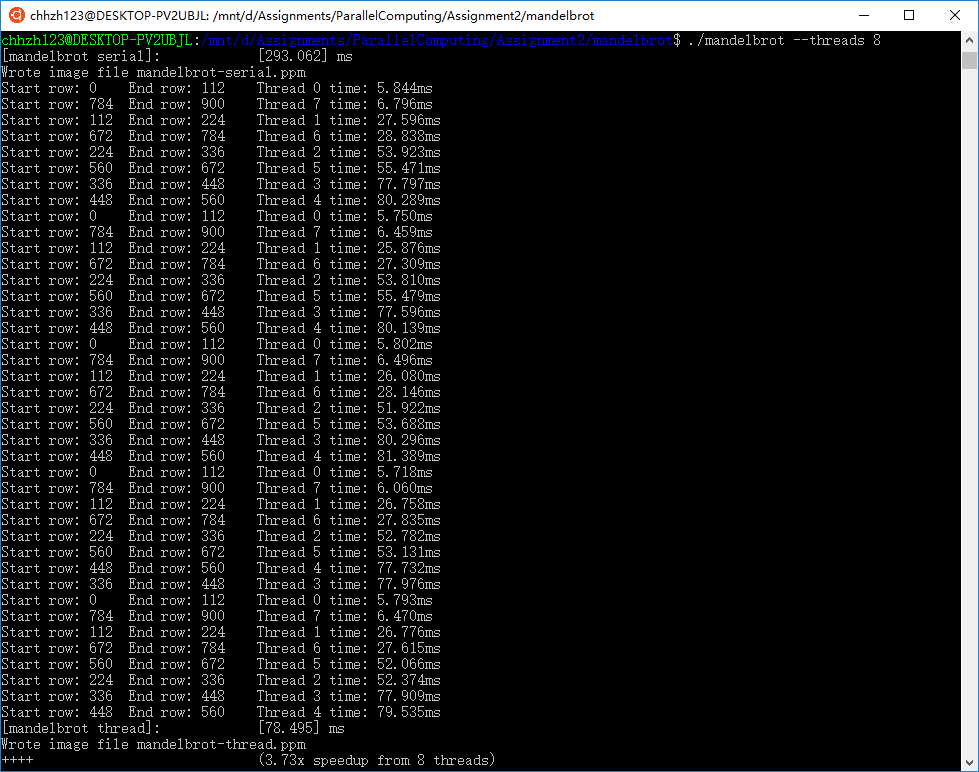
\includegraphics[width=0.7\linewidth]{fig/result.PNG}
\caption{Program output of 8 threads}
\label{fig:result}
\end{figure}

The speedup graph\footnote{This graph is created with Python Matplotlib, and the notebook \textit{plot.ipynb} is also in the attachment.} of different number of threads is shown in Fig.~\ref{fig:speedup}.
\begin{figure}[H]
\centering
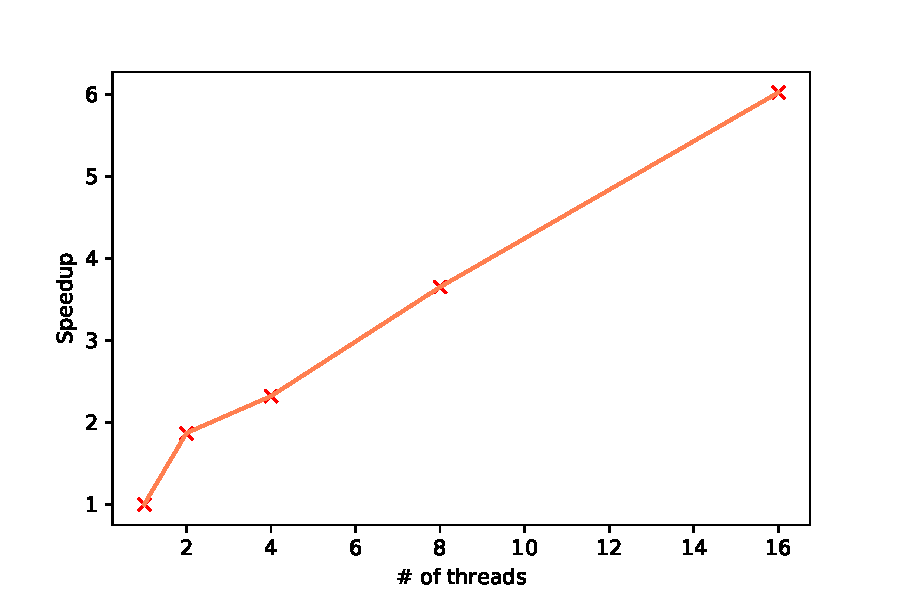
\includegraphics[width=0.5\linewidth]{fig/speedup.pdf}
\caption{Speedup of different number of threads}
\label{fig:speedup}
\end{figure}

From Fig.~\ref{fig:result}, we can clearly see the load imbalance that some threads terminate fast while others still work hard.
Nevertheless, all the threads work parallelly, and the total time is determined by the thread using the most time.

This experiment scales very well.
From Fig.~\ref{fig:speedup}, we can see that the speedup is almost linear to the number of threads.
The more threads, the faster execution.
However, the slope of this line is smaller than 1 due to the overheads of creating threads.

\end{document}